\section{内燃机}

%! src=60 kind=orig title=内燃机·章节导入
\begin{frame}[t,shrink]{\src{60}{内燃机：章节导入}}
\chapterintro{05}{内燃机}{Internal combustion engine: geometry, cycles and performance}
{\begin{itemize}
  \item 一个机体、两大机构、五大系统分别是什么？
  \item 止点、行程、排量、压缩比之间怎样联系？
  \item 四冲程与二冲程如何工作？性能参数怎样定义？
\end{itemize}}
{原页 60--72 \,$\cdot$\, 主线：结构 $\rightarrow$ 几何 $\rightarrow$ 工作循环 $\rightarrow$ 性能}
\vspace{3mm}
\begin{center}
\small
\textbf{关键词}\quad 曲柄连杆 \enspace$\cdot$\enspace 压缩比 \enspace$\cdot$\enspace 四冲程 \enspace$\cdot$\enspace 有效功率 \enspace$\cdot$\enspace 燃油消耗率
\end{center}
\end{frame}

%! src=61 kind=orig title=内燃机的定义与分类
\begin{frame}[t,shrink]{\src{61}{内燃机的定义与分类}}
内燃机使燃料在机器内部燃烧，把释放的热能直接转换为机械功；课件主要讨论\textbf{活塞式内燃机}。
\begin{smalltab}
\begin{tabularx}{\linewidth}{@{}>{\bfseries}p{25mm}p{40mm}X@{}}
  \toprule
  分类依据 & 类型 & 说明\\
  \midrule
  点火方式 & 点燃式、压燃式 & 火花塞点火 / 压缩自燃\\
  冲程数 & 二冲程、四冲程 & 一个循环对应的曲轴转数不同\\
  燃料 & 汽油机、柴油机、煤气机 & 燃料与混合方式不同\\
  \bottomrule
\end{tabularx}
\end{smalltab}
\begin{columns}[T,onlytextwidth]
\begin{column}{0.51\textwidth}
  \begin{itemize}
    \item 汽油机、柴油机是最常见的活塞式内燃机。
    \item 点火方式、冲程数、燃料类别是不同维度，不能相互替代。
    \item “内燃”指燃烧发生在机器内部，不是指燃料在气缸外预燃。
  \end{itemize}
\end{column}
\begin{column}{0.46\textwidth}
  \begin{keybox}{分类示例}
  \small 一台“四冲程、压燃式、柴油机”同时用了三个分类维度；回答时要分别说明。
  \end{keybox}
\end{column}
\end{columns}
\end{frame}

%! src=62 kind=orig title=一个机体、两大机构、五大系统
\begin{frame}[t,shrink]{\src{62}{一个机体、两大机构、五大系统}}
\begin{columns}[T,onlytextwidth]
\begin{column}{0.51\textwidth}
  \begin{itemize}
    \item \textbf{一个机体}：安装、支承各部件，形成气缸与曲轴箱。
    \item \textbf{曲柄连杆机构}：把活塞往复运动变为曲轴转动。
    \item \textbf{配气机构}：控制进、排气门的开启与关闭。
    \item \textbf{五大系统}：燃料供给、点火、润滑、冷却、启动。
  \end{itemize}
\end{column}
\begin{column}{0.46\textwidth}
  \begin{keybox}{结构层级}
  \small 机体是基础件；两大机构传递运动和换气；五大系统保障燃料、着火、润滑、散热和启动。
  \end{keybox}
  \vspace{0.8mm}
  \begin{amberbox}{机型差异}
  \small 柴油机依靠压燃，通常不设汽油机式火花点火系统；“五大系统”是通用框架，具体配置随机型而变。
  \end{amberbox}
\end{column}
\end{columns}
\vspace{1mm}
\begin{center}
\begin{tikzpicture}[x=1mm,y=1mm,scale=0.9,transform shape]
  \node[box,text width=22mm] (body) at (12,0) {机体};
  \node[box,text width=29mm] (mech) at (50,8) {曲柄连杆机构};
  \node[box,text width=27mm] (valve) at (50,-8) {配气机构};
  \node[boxb,text width=31mm] (sys) at (95,0) {燃料 / 点火 / 润滑 / 冷却 / 启动};
  \draw[arr] (body) -- (mech);
  \draw[arr] (body) -- (valve);
  \draw[arr] (mech) -- (sys);
  \draw[arr] (valve) -- (sys);
\end{tikzpicture}
\end{center}
\end{frame}

%! src=62 kind=supp title=从结构图联系机构与系统
\begin{frame}[t,shrink]{\srcsupp{62}{从结构图联系两大机构与五大系统}}
\begin{columns}[T,onlytextwidth]
\begin{column}{0.37\textwidth}
  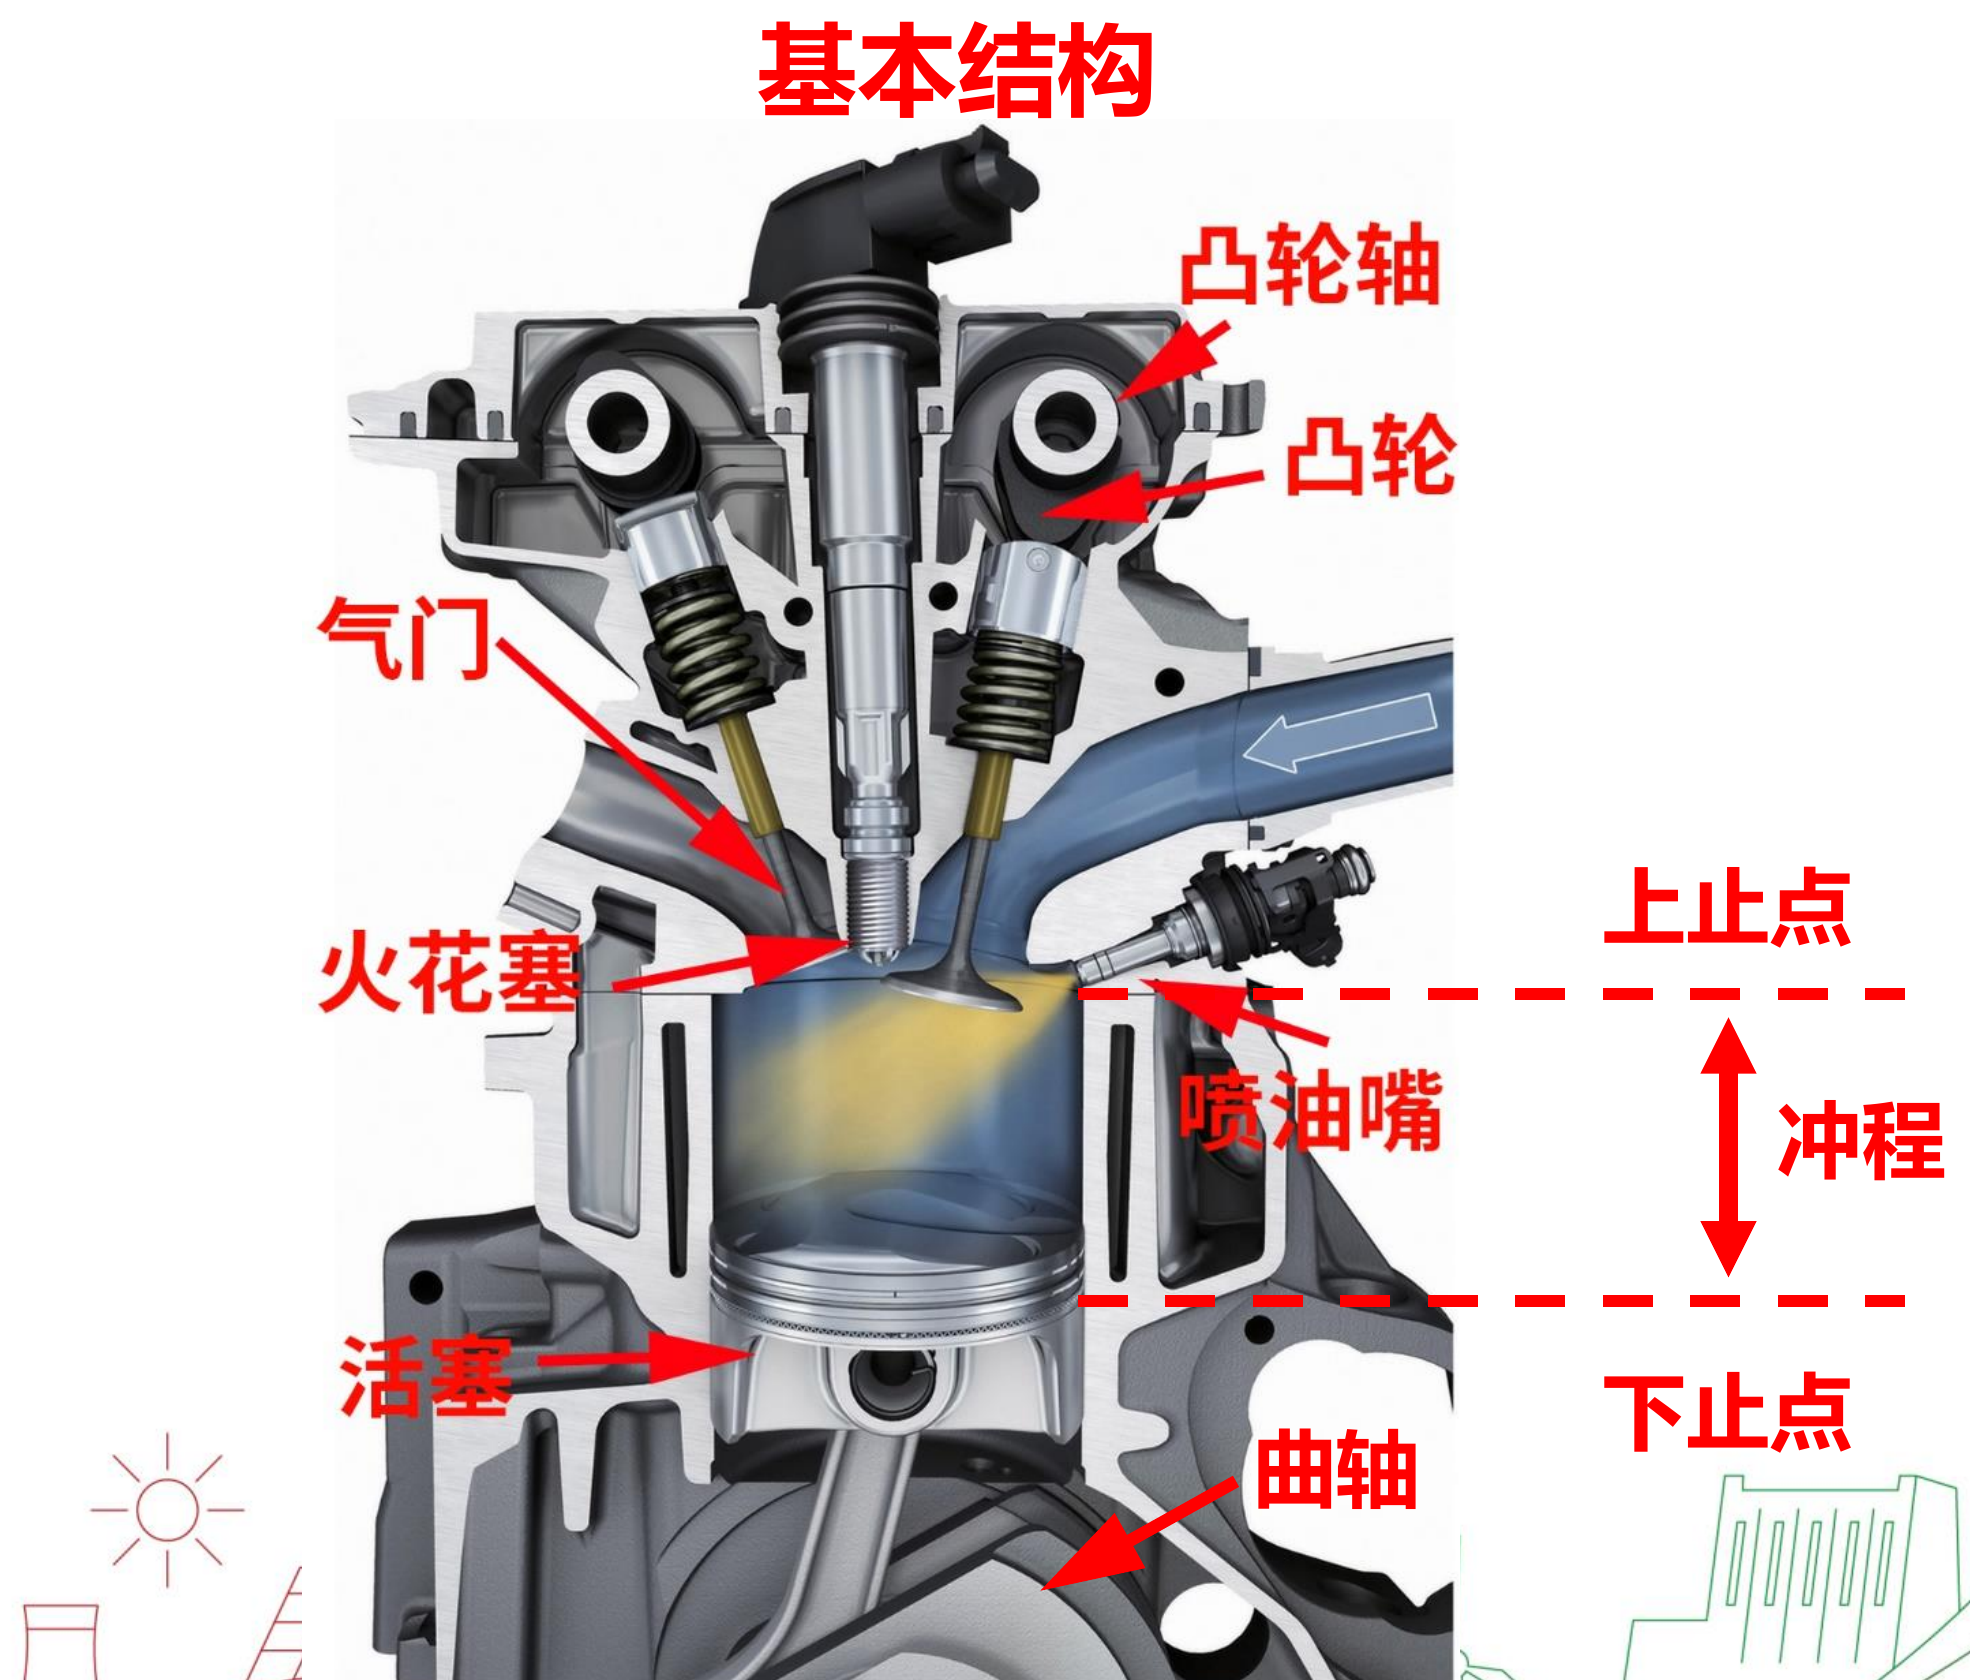
\includegraphics[height=46mm,keepaspectratio]{figures/course/engine_structure.png}
  \figcap{原课件第 62 页结构图局部；已保留主要标注。}
\end{column}
\begin{column}{0.59\textwidth}
  \begin{itemize}
    \item 活塞、连杆、曲轴：承受气体力，形成旋转输出。
    \item 凸轮轴、气门：控制换气时序。
    \item 火花塞 / 喷油器：对应点燃或压燃、缸外或缸内供油。
    \item 冷却、润滑：保障温度与摩擦状态。
  \end{itemize}
  \vspace{0.5mm}
  \begin{keybox}{读图顺序}
  \small 先找活塞—连杆—曲轴的运动链，再找凸轮—气门的换气链，最后看燃料与点火装置。
  \end{keybox}
\end{column}
\end{columns}
\end{frame}

%! src=63 kind=orig title=上、下止点与活塞行程
\begin{frame}[t,shrink]{\src{63}{上、下止点与活塞行程}}
\begin{columns}[T,onlytextwidth]
\begin{column}{0.50\textwidth}
  \begin{itemize}
    \item \textbf{上止点}：活塞顶离曲轴回转中心最远的位置。
    \item \textbf{下止点}：活塞顶离曲轴回转中心最近的位置。
    \item 在上、下止点处，活塞瞬时速度为零。
    \item 活塞行程 \(S\)：上、下止点之间的距离；曲柄半径为 \(R\)。
  \end{itemize}
  \vspace{0.5mm}
  \begin{keybox}{几何关系}
  \small 对于气缸中心线通过曲轴回转中心的机构：
  $$
  S=2R
  $$
  \end{keybox}
\end{column}
\begin{column}{0.47\textwidth}
\begin{center}
\begin{tikzpicture}[x=1mm,y=1mm,scale=0.9,transform shape]
  \draw[thick,black!55] (0,0) rectangle (20,38);
  \fill[black!25] (2,31) rectangle (18,34);
  \fill[black!10] (2,9) rectangle (18,12);
  \draw[<->,thin] (24,9) -- (24,34);
  \node[lab,anchor=west] at (24.5,21.5) {\(S\)};
  \draw[dashline] (18,34) -- (26,34);
  \draw[dashline] (18,9) -- (26,9);
  \node[lab,anchor=west] at (26,34) {上止点};
  \node[lab,anchor=west] at (26,9) {下止点};
  \draw[thick,black!55] (10,-4) circle (5);
  \draw[thick,black!55] (10,-4) -- (10,9);
  \draw[thick,cprimary] (10,-4) -- (15,-4);
  \node[lab,text=cprimary,anchor=south] at (13,-4) {\(R\)};
  \node[lab,anchor=north] at (10,-10) {曲柄半径 \(R\)};
\end{tikzpicture}
\end{center}
\figcap{活塞在上、下止点之间移动的距离为行程 \(S\)。}
\end{column}
\end{columns}
\end{frame}

%! src=63 kind=supp title=行程、转速与平均活塞速度
\begin{frame}[t,shrink]{\srcsupp{63}{行程、转速与平均活塞速度}}
曲轴每转一周，活塞累计移动距离为 \(2S\)，因此：
$$
\bar c_{\mathrm{p}}=\frac{2Sn}{60}
$$
\begin{columns}[T,onlytextwidth]
\begin{column}{0.51\textwidth}
  \begin{itemize}
    \item \(S\) 用 \(\mathrm{m}\)，\(n\) 用 \(\mathrm{r/min}\)，平均活塞速度为 \(\mathrm{m/s}\)。
    \item 平均速度概括运动强度；瞬时速度随曲轴转角变化。
    \item 止点处瞬时速度为零，不代表平均速度为零。
    \item 行程对应直线运动，转速对应曲轴转动，必须通过机构关系联系。
  \end{itemize}
\end{column}
\begin{column}{0.46\textwidth}
  \begin{keybox}{补充算例}
  \small 取 \(S=90\,\mathrm{mm}=0.09\,\mathrm{m}\)，\(n=3000\,\mathrm{r/min}\)：
  $$
  \bar c_{\mathrm{p}}=\frac{2\times0.09\times3000}{60}=9\,\mathrm{m/s}
  $$
  \end{keybox}
  \vspace{0.6mm}
  \begin{amberbox}{边界}
  \small 这里的平均速度是“累计路程/时间”，不是往复周期内平均速度矢量。
  \end{amberbox}
\end{column}
\end{columns}
\end{frame}

%! src=64 kind=orig title=工作容积、排量与燃烧室容积
\begin{frame}[t,shrink]{\src{64}{工作容积、排量与燃烧室容积}}
\begin{columns}[T,onlytextwidth]
\begin{column}{0.52\textwidth}
  \begin{smalltab}
  \begin{tabularx}{\linewidth}{@{}>{\bfseries}p{26mm}X@{}}
    \toprule
    名称 & 含义\\
    \midrule
    气缸工作容积 \(V_{\mathrm{s}}\) & 活塞从上止点移到下止点扫过的容积\\
    内燃机排量 \(V_{\mathrm{disp}}\) & 所有气缸工作容积之和\\
    燃烧室容积 \(V_{\mathrm{c}}\) & 活塞在上止点时，活塞顶以上的剩余容积\\
    \bottomrule
  \end{tabularx}
  \end{smalltab}
  \vspace{0.6mm}
  $$
  V_{\mathrm{s}}=\frac{\pi D^2}{4}S,
  \qquad
  V_{\mathrm{disp}}=zV_{\mathrm{s}}
  $$
  \begin{itemize}
    \item \(D\) 为缸径，\(z\) 为气缸数。
    \item 排量不包含燃烧室容积。
  \end{itemize}
\end{column}
\begin{column}{0.45\textwidth}
\begin{center}
\begin{tikzpicture}[x=1mm,y=1mm,scale=0.9,transform shape]
  \draw[thick,black!55] (0,0) rectangle (28,50);
  \fill[cblue!28] (0,45) rectangle (28,50);
  \fill[cprimary!18] (0,20) rectangle (28,45);
  \fill[black!30] (1,20) rectangle (27,24);
  \draw[dashline] (0,45) -- (28,45);
  \node[lab,anchor=west] at (29,47.5) {\(V_{\mathrm{c}}\)};
  \node[lab,anchor=west] at (29,32) {\(V_{\mathrm{s}}\)};
  \node[lab,anchor=west] at (29,21) {活塞};
  \node[lab,anchor=north] at (14,-2) {下止点位置};
\end{tikzpicture}
\end{center}
\figcap{气缸工作容积是活塞扫过的圆柱体积；燃烧室容积在活塞上止点以上。}
\end{column}
\end{columns}
\end{frame}

%! src=64 kind=supp title=用几何关系检查排量与单位
\begin{frame}[t,shrink]{\srcsupp{64}{用几何关系检查排量与单位}}
$$
V_{\mathrm{s}}=\frac{\pi D^2S}{4},
\qquad
V_{\mathrm{disp}}=z\frac{\pi D^2S}{4}
$$
\begin{columns}[T,onlytextwidth]
\begin{column}{0.51\textwidth}
  \begin{itemize}
    \item 缸径平方乘行程，因此同时放大缸径和行程，会显著改变排量。
    \item 缸径、行程必须先统一长度单位，再计算容积。
    \item \(1\,\mathrm{L}=10^{-3}\,\mathrm{m^3}=10^3\,\mathrm{cm^3}\)。
    \item 排量是几何参数，功率还取决于转速、充气与每循环输出功。
  \end{itemize}
\end{column}
\begin{column}{0.46\textwidth}
  \begin{keybox}{检查顺序}
  \small 先统一单位 $\rightarrow$ 算单缸 \(V_{\mathrm{s}}\) $\rightarrow$ 乘缸数得排量 $\rightarrow$ 再与压缩比所需的 \(V_{\mathrm{c}}\) 区分。
  \end{keybox}
  \vspace{0.6mm}
  \begin{amberbox}{符号}
  \small 这里的 \(D\) 是缸径；锅炉章节的 \(D\) 是蒸发量。跨章节阅读时要重新确认符号。
  \end{amberbox}
\end{column}
\end{columns}
\end{frame}

%! src=65 kind=orig title=气缸总容积与压缩比
\begin{frame}[t,shrink]{\src{65}{气缸总容积与压缩比}}
以 \(V_{\mathrm{c}}\) 表示燃烧室容积，\(V_{\mathrm{a}}\) 表示下止点时的总容积：
$$
V_{\mathrm{a}}=V_{\mathrm{s}}+V_{\mathrm{c}}
$$
$$
\varepsilon=\frac{V_{\mathrm{a}}}{V_{\mathrm{c}}}
=1+\frac{V_{\mathrm{s}}}{V_{\mathrm{c}}}
$$
\begin{columns}[T,onlytextwidth]
\begin{column}{0.47\textwidth}
  \begin{itemize}
    \item 压缩比 \(\varepsilon\) 是无量纲几何参数。
    \item 其他条件相同时，压缩比增大意味着压缩终了压力、温度更高。
    \item \textbf{压缩比是容积比}，不能直接当作压缩前后压力之比。
  \end{itemize}
\end{column}
\begin{column}{0.50\textwidth}
  \begin{keybox}{理想等熵关系}
  \small 若把缸内气体视为定比热理想气体，并近似为等熵压缩：
  $$
  \frac{T_2}{T_1}=\varepsilon^{\kappa-1},
  \qquad
  \frac{p_2}{p_1}=\varepsilon^{\kappa}
  $$
  这只是补充的理想模型，实际还受换热、泄漏和充气影响。
  \end{keybox}
\end{column}
\end{columns}
\end{frame}

%! src=66 kind=orig title=喷油与点火时序
\begin{frame}[t,shrink]{\src{66}{喷油与点火时序}}
\begin{center}
\begin{tikzpicture}[x=0.16mm,y=1mm,xshift=18mm]
  \fill[cblue!7] (0,2) rectangle (180,20);
  \fill[cprimary!7] (180,2) rectangle (360,20);
  \fill[camber!10] (360,2) rectangle (540,20);
  \fill[black!5] (540,2) rectangle (720,20);
  \foreach \y in {14,9,4}{\fill[white] (0,\y-1.2) rectangle (720,\y+1.2);}
  \foreach \y/\n in {14/气道喷射,9/缸内直喷,4/柴油机}{
    \node[lab,anchor=east] at (-2,\y) {\n};
  }
  \draw[thin,black!40] (0,2)--(720,2);
  \foreach \x in {180,360,540}{\draw[dashline] (\x,2)--(\x,20);}
  \node[lab,anchor=south] at (90,20) {进气};
  \node[lab,anchor=south] at (270,20) {压缩};
  \node[lab,anchor=south] at (450,20) {做功};
  \node[lab,anchor=south] at (630,20) {排气};
  % PFI
  \draw[cblue,thick] (30,12) -- (30,16);
  \draw[cprimary,thick] (350,12) -- (350,16);
  % GDI
  \draw[cblue,thick] (320,7) -- (320,11);
  \draw[cprimary,thick] (350,7) -- (350,11);
  % Diesel
  \draw[camber,thick] (340,2) -- (340,6);
  \foreach \x/\t in {0/0,180/180,360/360,540/540,720/720}{
    \draw[thin] (\x,2)--(\x,1);
    \node[lab,anchor=north] at (\x,1) {\t};
  }
  \node[lab,anchor=north] at (360,-5) {曲轴转角 / \((^\circ)\)};
\end{tikzpicture}
\end{center}
\begin{columns}[T,onlytextwidth]
\begin{column}{0.55\textwidth}
  \begin{itemize}
    \item 气道喷射汽油机：燃油在气道形成混合气，进气过程带入气缸，压缩末期火花点火。
    \item 缸内直喷汽油机：燃油直接喷入气缸，图示在压缩阶段，仍需火花点火。
    \item 柴油机：先压缩空气，压缩末期喷油，依靠高温空气压燃（不设火花塞）。
  \end{itemize}
\end{column}
\begin{column}{0.42\textwidth}
  \begin{keybox}{图例}
  \small \textcolor{cblue}{\rule{2mm}{1.6pt}} 喷油；\quad
  \textcolor{cprimary}{\rule{2mm}{1.6pt}} 火花点火；\quad
  \textcolor{camber}{\rule{2mm}{1.6pt}} 柴油喷油。
  \par\vspace{1mm}
  实际时刻随转速、负荷和排放策略变化，图中位置只是示意。
  \end{keybox}
\end{column}
\end{columns}
\end{frame}

%! src=67 kind=orig title=四冲程工作循环
\begin{frame}[t,shrink]{\src{67}{四冲程工作循环}}
\begin{columns}[T,onlytextwidth]
\begin{column}{0.60\textwidth}
  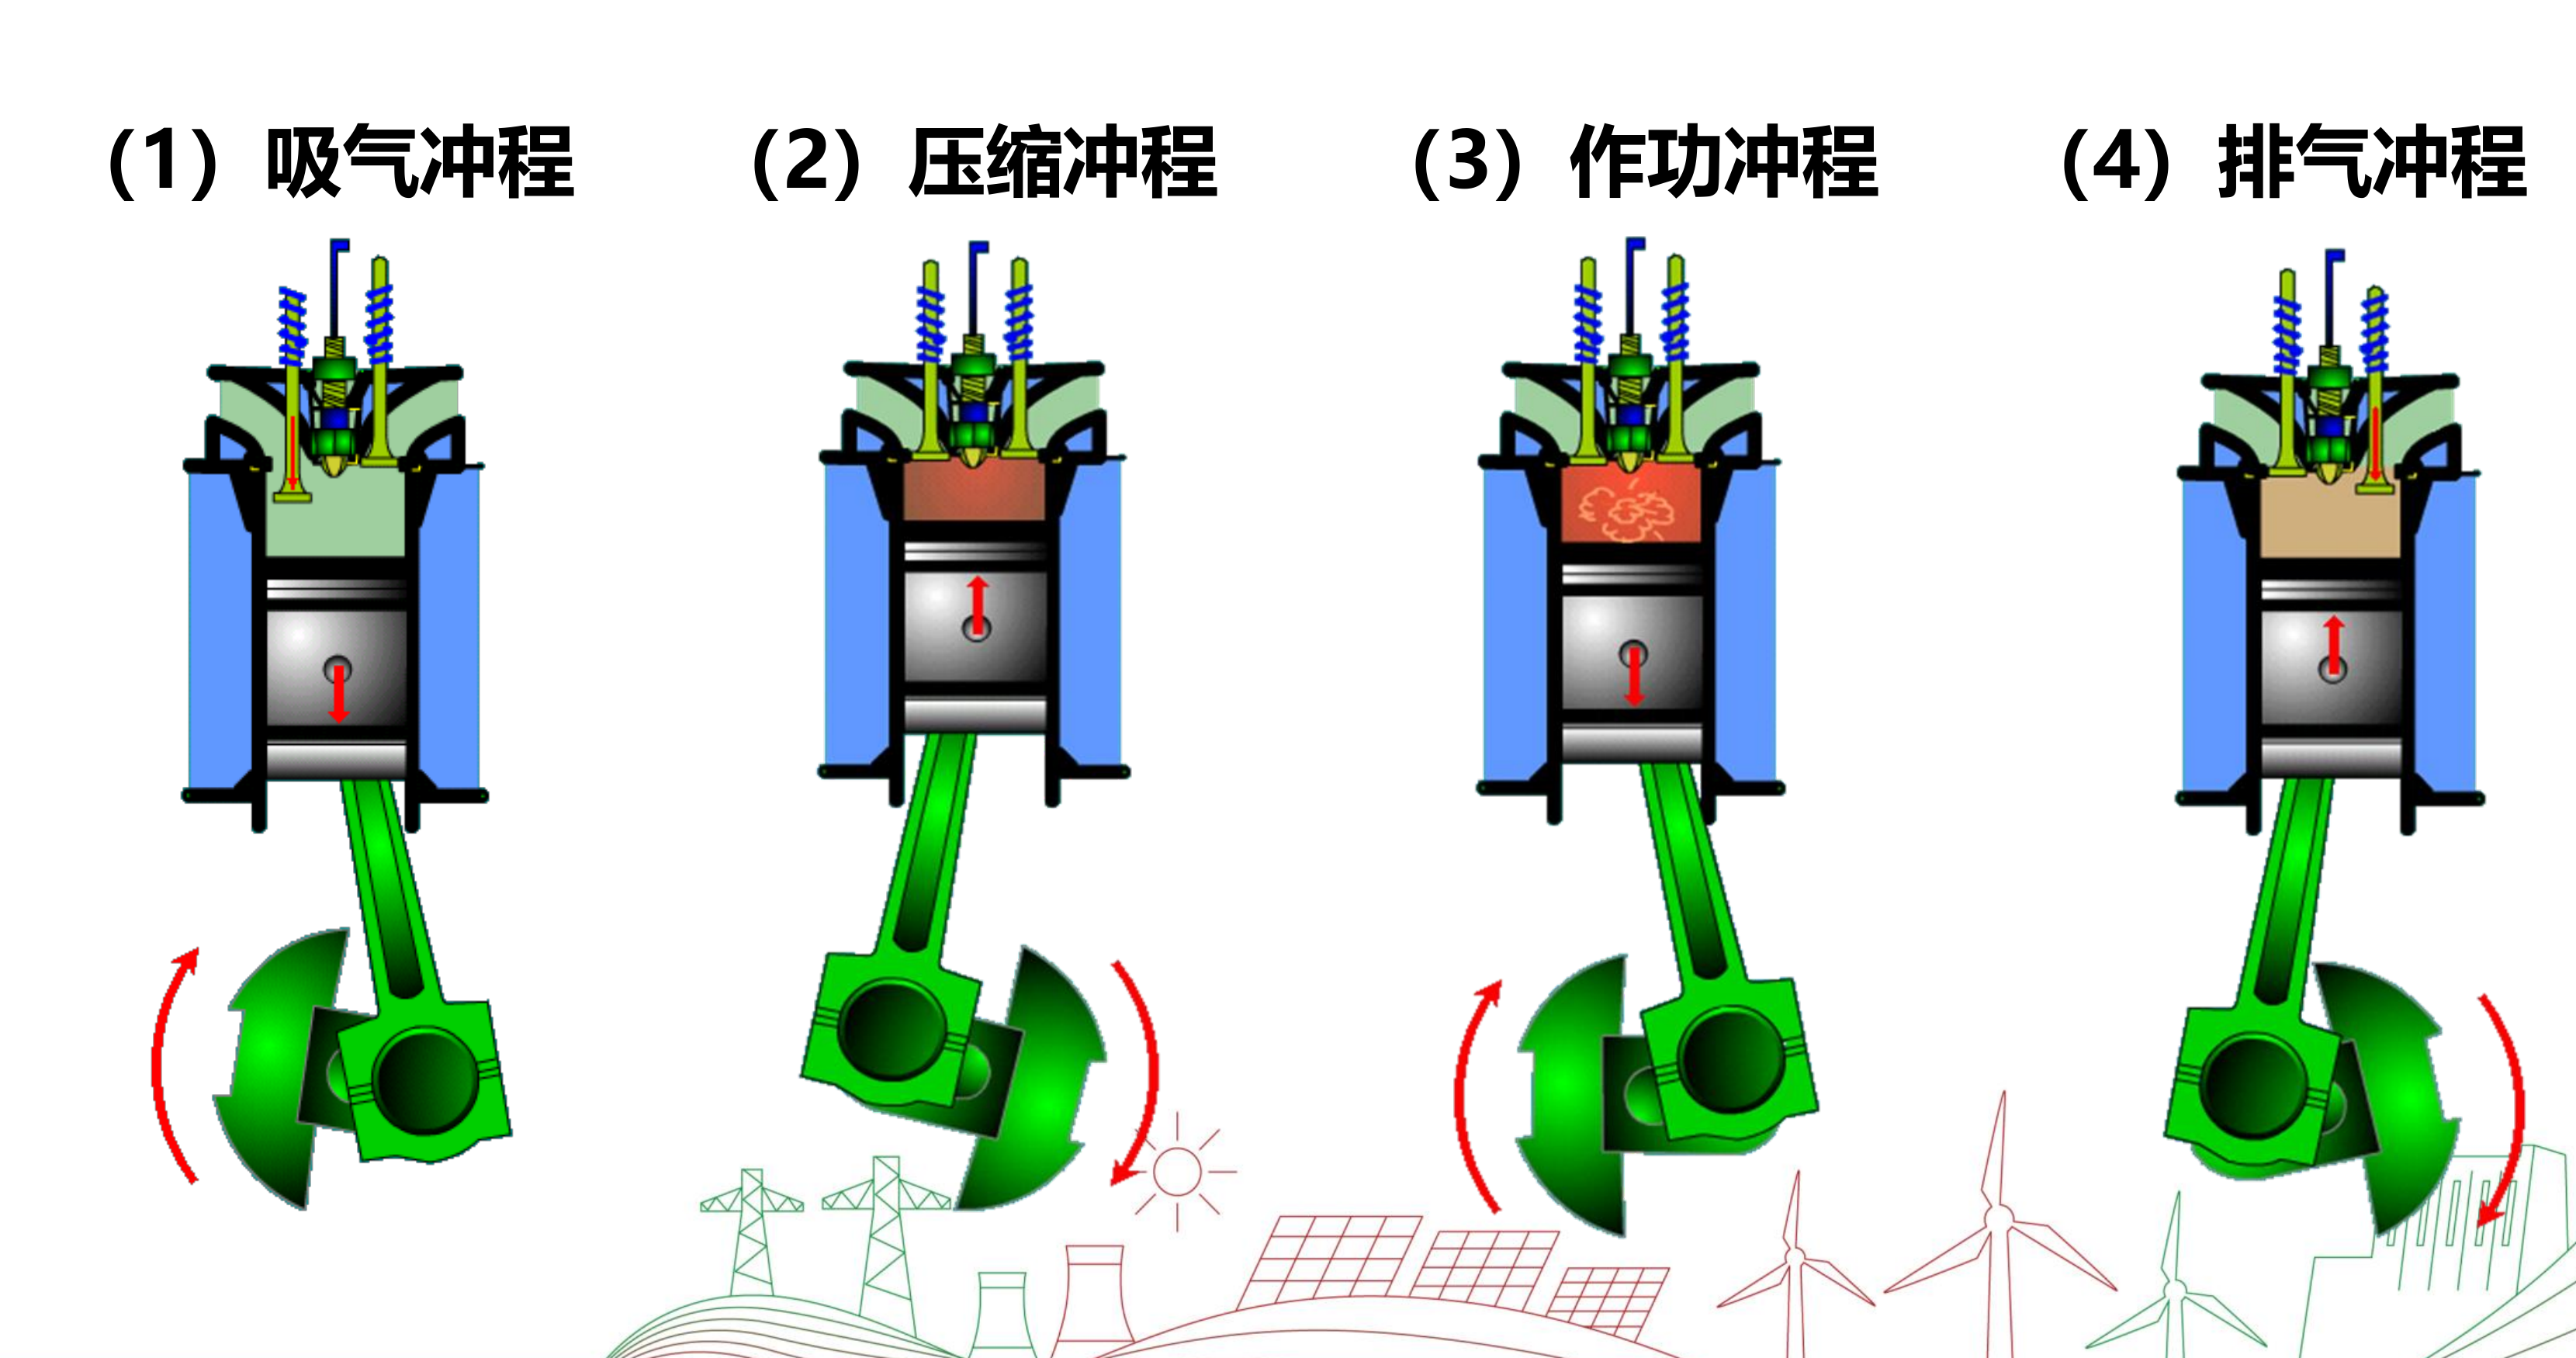
\includegraphics[width=\linewidth]{figures/course/four_stroke.png}
  \figcap{原课件第 67 页四冲程示意图；已保留四个冲程标题。}
\end{column}
\begin{column}{0.37\textwidth}
  \begin{smalltab}
  \begin{tabularx}{\linewidth}{@{}>{\bfseries}p{11mm}X@{}}
    \toprule
    冲程 & 主要过程\\
    \midrule
    进气 & 进气门开，吸入新鲜充量\\
    压缩 & 气门关，压缩气体\\
    做功 & 燃烧膨胀，推动活塞\\
    排气 & 排气门开，排出废气\\
    \bottomrule
  \end{tabularx}
  \end{smalltab}
  \begin{itemize}
    \item 一个循环曲轴转两周，即 \(720^\circ\)。
    \item 每缸每循环做功一次。
  \end{itemize}
\end{column}
\end{columns}
\end{frame}

%! src=67 kind=supp title=四冲程的做功频率
\begin{frame}[t,shrink]{\srcsupp{67}{四冲程的做功频率}}
每缸每两转完成一个工作循环。转速为 \(n\,\mathrm{r/min}\) 时：
$$
f_{\mathrm{cycle}}=\frac{n}{120}\,\mathrm{s^{-1}}
$$
若每缸每循环有效功为 \(W_{\mathrm{e,cyc}}\)，缸数为 \(z\)：
$$
P_{\mathrm{e}}=zW_{\mathrm{e,cyc}}\frac{n}{120}
$$
\begin{columns}[T,onlytextwidth]
\begin{column}{0.50\textwidth}
  \begin{itemize}
    \item \(W_{\mathrm{e,cyc}}\) 用 \(\mathrm{J}\)，所得 \(P_{\mathrm{e}}\) 为 \(\mathrm{W}\)。
    \item 四冲程每缸每两转做功一次；二冲程每转一次。
    \item 做功频率加倍不意味着同尺寸、同转速下功率必然严格加倍。
  \end{itemize}
\end{column}
\begin{column}{0.47\textwidth}
  \begin{keybox}{曲轴转角}
  \small 四冲程：进气 \(0\sim180^\circ\)，压缩 \(180\sim360^\circ\)，做功 \(360\sim540^\circ\)，排气 \(540\sim720^\circ\)（理想化划分）。
  \end{keybox}
\end{column}
\end{columns}
\end{frame}

%! src=68 kind=orig title=二冲程工作循环
\begin{frame}[t,shrink]{\src{68}{二冲程工作循环}}
\begin{columns}[T,onlytextwidth]
\begin{column}{0.60\textwidth}
  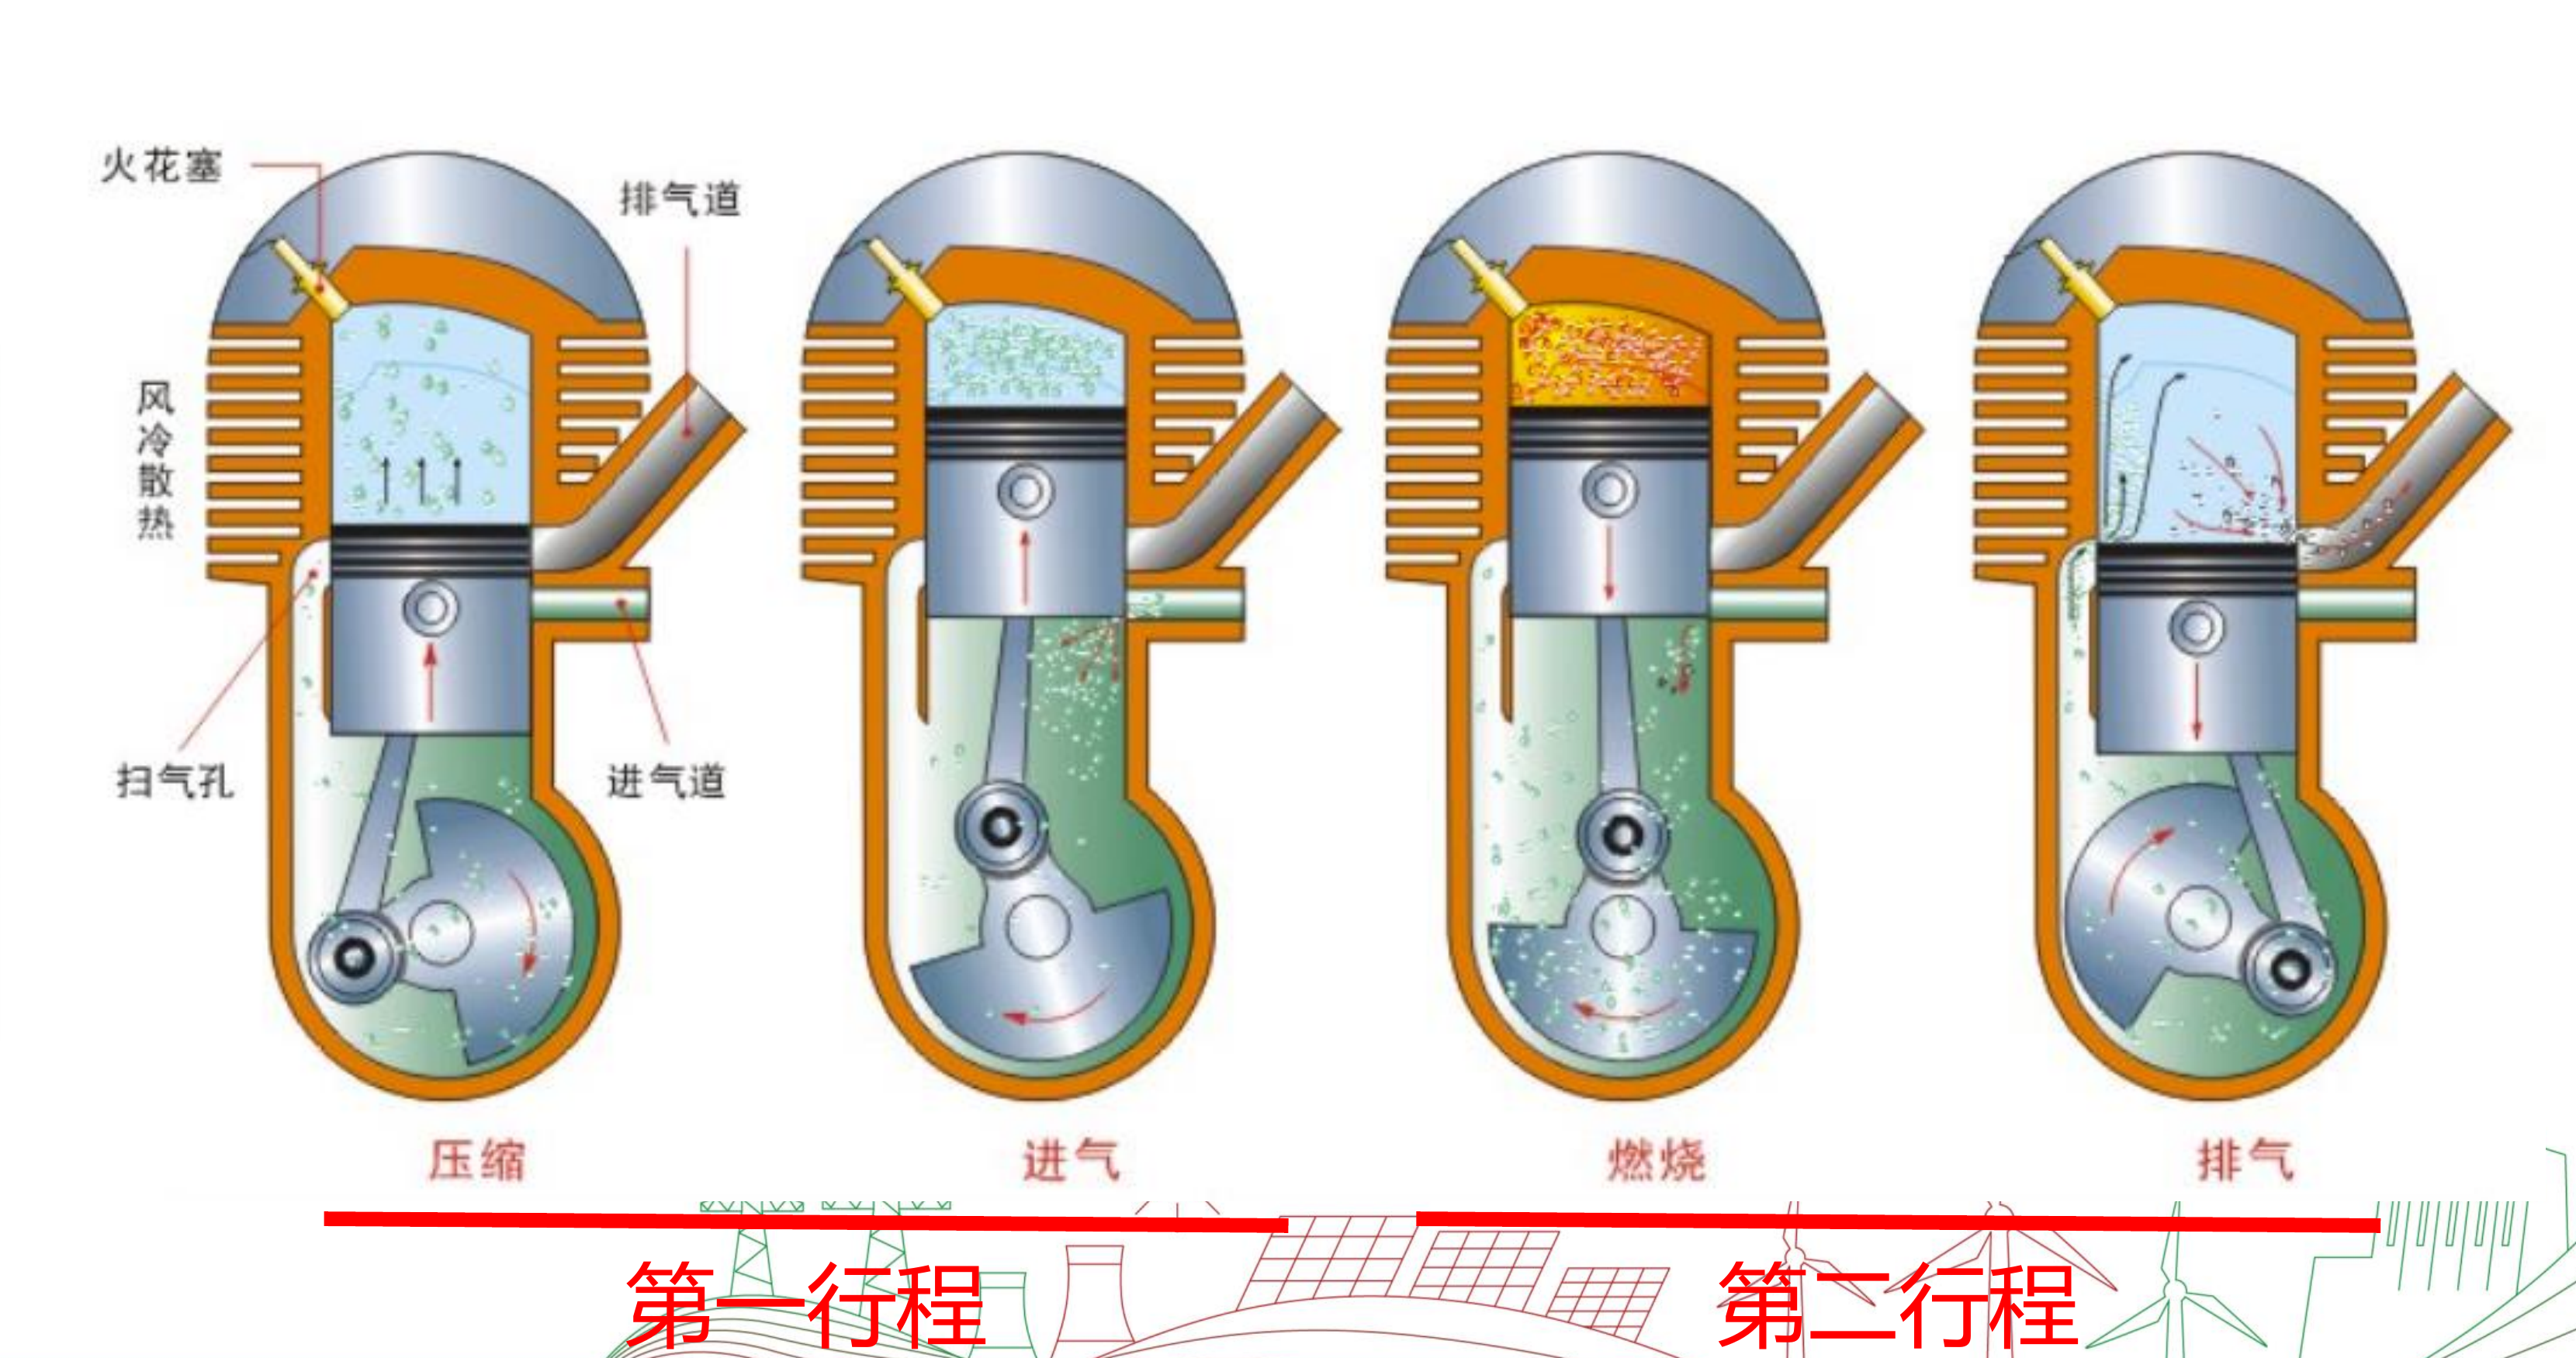
\includegraphics[width=\linewidth]{figures/course/two_stroke.png}
  \figcap{原课件第 68 页二冲程示意图；进排气口与扫气孔同时可见。}
\end{column}
\begin{column}{0.37\textwidth}
  \begin{itemize}
    \item 第一行程，活塞上行：缸内混合气压缩，曲轴箱吸入新鲜混合气。
    \item 上止点附近点火燃烧，进入第二行程。
    \item 第二行程，活塞下行：燃气膨胀做功，曲轴箱内充量受压。
    \item 下止点附近排气口、扫气口相继开启，进行排气与扫气。
    \item 一个循环曲轴转一周，即 \(360^\circ\)。
  \end{itemize}
\end{column}
\end{columns}
\end{frame}

%! src=68 kind=supp title=二冲程的扫气与循环重叠
\begin{frame}[t,shrink]{\srcsupp{68}{二冲程的扫气与循环重叠}}
\begin{itemize}
  \item 上行：缸内压缩，同时曲轴箱吸入新鲜充量；下行：膨胀做功，同时为后续扫气准备充量。
  \item 下止点附近：排气与扫气在相近时段发生；每缸每转一个循环，频率为 \(n/60\)。
  \item 二冲程的换气与其他过程重叠；图示结构不能概括所有二冲程发动机（如直流扫气、回流扫气等）。
\end{itemize}
\begin{center}
\begin{tikzpicture}[x=0.32mm,y=1.4mm]
  \fill[cprimary!15] (0,0.5) rectangle (160,4.5);
  \fill[camber!18] (160,0.5) rectangle (220,4.5);
  \fill[cblue!12] (220,0.5) rectangle (360,4.5);
  \draw[thin] (0,0.5) rectangle (360,4.5);
  \node[lab] at (80,6.1) {膨胀};
  \node[lab] at (190,6.1) {排气 / 扫气重叠};
  \node[lab] at (290,6.1) {压缩};
  \draw[thin] (160,0.5)--(160,7);
  \draw[thin] (220,0.5)--(220,7);
  \draw[axis] (0,0) -- (370,0);
  \foreach \x/\t in {0/0,180/180,360/360}{\draw[thin] (\x,0)--(\x,-1);\node[lab,anchor=north] at (\x,-1) {\t};}
  \node[lab,anchor=north] at (180,-6) {曲轴转角 / \((^\circ)\)};
\end{tikzpicture}
\end{center}
\figcap{补充时序示意：换气与膨胀/压缩存在重叠，不对应具体发动机配气时刻。}
\end{frame}

%! src=69 kind=orig title=汽油机与柴油机比较
\begin{frame}[t,shrink]{\src{69}{汽油机与柴油机比较}}
本页比较对象是典型\textbf{四冲程}汽油机与柴油机。
\begin{smalltab}
\begin{tabularx}{\linewidth}{@{}>{\bfseries}p{30mm}XX@{}}
  \toprule
  项目 & 汽油机 & 柴油机\\
  \midrule
  典型关键部件 & 火花塞 & 喷油器\\
  进气内容 & 传统气道供油时为混合气 & 主要为空气\\
  点火方式 & 点燃式 & 压燃式\\
  课件压缩比示例 & \(8\sim11\) & \(13\sim18\)\\
  每缸工作循环 & 四冲程、两周、做功一次 & 四冲程、两周、做功一次\\
  \bottomrule
\end{tabularx}
\end{smalltab}
\begin{columns}[T,onlytextwidth]
\begin{column}{0.53\textwidth}
  \begin{itemize}
    \item 缸内直喷汽油机的进气应结合第 66 页理解，不能套用“都吸入混合气”。
    \item 课件将优点简写为汽油机轻便、柴油机便宜且功率大；这些比较依具体机型而变。
  \end{itemize}
\end{column}
\begin{column}{0.44\textwidth}
  \begin{amberbox}{压缩比不是唯一判据}
  \small 压缩比、燃料性质、喷射方式和排放控制共同决定机型差异，不能只看一个数字。
  \end{amberbox}
\end{column}
\end{columns}
\end{frame}

%! src=70 kind=orig title=有效转矩与有效功率
\begin{frame}[t,shrink]{\src{70}{有效转矩与有效功率}}
\begin{columns}[T,onlytextwidth]
\begin{column}{0.51\textwidth}
  \begin{itemize}
    \item \textbf{有效转矩} \(T_{\mathrm{e}}\)：克服摩擦、附件驱动等损失后，曲轴输出的净转矩，单位 \(\mathrm{N\cdot m}\)。
    \item \textbf{有效功率} \(P_{\mathrm{e}}\)：曲轴或飞轮对外输出的净功率，单位 \(\mathrm{kW}\)。
    \item 功率等于转矩乘角速度，测得转矩和转速后即可计算。
  \end{itemize}
\end{column}
\begin{column}{0.46\textwidth}
  \begin{keybox}{基本关系}
  \small
  $$
  P_{\mathrm{e}}=T_{\mathrm{e}}\omega,
  \qquad
  \omega=\frac{2\pi n}{60}
  $$
  常用单位：
  $$
  \frac{P_{\mathrm{e}}}{\mathrm{kW}}
  \approx\frac{1}{9550}
  \left(\frac{T_{\mathrm{e}}}{\mathrm{N\cdot m}}\right)
  \left(\frac{n}{\mathrm{r/min}}\right)
  $$
  \end{keybox}
\end{column}
\end{columns}
\vspace{0.5mm}
\begin{amberbox}{区分“指示”和“有效”}
\small 指示功率是缸内气体对活塞做功的功率；有效功率是扣除机械损失后从曲轴输出的功率。
\end{amberbox}
\end{frame}

%! src=70 kind=supp title=9550 系数从哪里来
\begin{frame}[t,shrink]{\srcsupp{70}{9550 系数从哪里来}}
当 \(n\) 用 \(\mathrm{r/min}\)，\(T_{\mathrm{e}}\) 用 \(\mathrm{N\cdot m}\) 时：
$$
P_{\mathrm{e}}\,[\mathrm{W}]
=T_{\mathrm{e}}\frac{2\pi n}{60}
$$
$$
P_{\mathrm{e}}\,[\mathrm{kW}]
=\frac{T_{\mathrm{e}}n}{60\times1000/(2\pi)}
\approx\frac{T_{\mathrm{e}}n}{9550}
$$
\begin{columns}[T,onlytextwidth]
\begin{column}{0.50\textwidth}
  \begin{itemize}
    \item \(60\) 把每分钟换为每秒；\(1000\) 把瓦换为千瓦。
    \item \(60\times1000/(2\pi)=9549.3\ldots\)，工程上取 9550。
    \item 转矩大不一定功率大，还要看转速。
  \end{itemize}
\end{column}
\begin{column}{0.47\textwidth}
  \begin{amberbox}{单位陷阱}
  \small 使用角速度 \(\omega\) 时，直接用 \(P=T\omega\)，不要再除以 9550；9550 只适用于 \(\mathrm{N\cdot m}\)、\(\mathrm{r/min}\)、\(\mathrm{kW}\) 这组单位。
  \end{amberbox}
\end{column}
\end{columns}
\end{frame}

%! src=71 kind=orig title=热效率与有效燃油消耗率
\begin{frame}[t,shrink]{\src{71}{热效率与有效燃油消耗率}}
$$
\eta_{\mathrm{t}}=\frac{P_{\mathrm{i}}}{\dot m_{\mathrm{f}}H_{\mathrm{u}}},
\qquad
\eta_{\mathrm{e}}=\frac{P_{\mathrm{e}}}{\dot m_{\mathrm{f}}H_{\mathrm{u}}}
$$
\begin{columns}[T,onlytextwidth]
\begin{column}{0.50\textwidth}
  \begin{itemize}
    \item 课件用 \(\eta_{\mathrm{t}}\) 表示\textbf{指示热效率}：燃料热量转为缸内指示功的比例。
    \item 有效热效率：转为曲轴有效功的比例，计入机械损失后更低。
    \item \(\dot m_{\mathrm{f}}\)：燃油质量流量；\(H_{\mathrm{u}}\)：低位发热量。
  \end{itemize}
\end{column}
\begin{column}{0.47\textwidth}
  \begin{keybox}{有效燃油消耗率}
  \small
  $$
  \frac{g_{\mathrm{e}}}{\mathrm{g/(kW\cdot h)}}
  =3.6\times10^6
  \frac{\dot m_{\mathrm{f}}/\mathrm{(kg/s)}}{P_{\mathrm{e}}/\mathrm{kW}}
  $$
  \end{keybox}
\end{column}
\end{columns}
\vspace{0.5mm}
\begin{amberbox}{符号提醒}
\small 原课件用 \(\eta_{\mathrm{t}}\) 指“指示热效率”，下标容易与温度 \(t\) 混淆；本整理在补充中改用 \(\eta_{\mathrm{i}}\) 表示同一含义。
\end{amberbox}
\end{frame}

%! src=71 kind=supp title=指示效率、有效效率与油耗率
\begin{frame}[t,shrink]{\srcsupp{71}{指示效率、有效效率与油耗率的关系}}
定义机械效率 \(\eta_{\mathrm{m}}=P_{\mathrm{e}}/P_{\mathrm{i}}\)，有：
$$
\eta_{\mathrm{e}}=\eta_{\mathrm{i}}\eta_{\mathrm{m}},
\qquad
\frac{g_{\mathrm{e}}}{\mathrm{g/(kW\cdot h)}}
=\frac{3.6\times10^6}
{\eta_{\mathrm{e}}\left(H_{\mathrm{u}}/\mathrm{(kJ/kg)}\right)}
$$
\begin{columns}[T,onlytextwidth]
\begin{column}{0.50\textwidth}
  \begin{itemize}
    \item 第一式区分缸内指示功与曲轴有效功，是定义的直接结果。
    \item 第二式在油耗用 \(\mathrm{g/(kW\cdot h)}\)、低位热值用 \(\mathrm{kJ/kg}\) 时成立。
    \item 同一种燃料下，油耗率降低对应有效热效率提高。
    \item 比较不同燃料时应先考虑低位热值，不能只比较质量油耗率。
  \end{itemize}
\end{column}
\begin{column}{0.46\textwidth}
  \begin{keybox}{量纲检查}
  \small \(g_{\mathrm{e}}H_{\mathrm{u}}\) 的单位为 \(\mathrm{g\cdot kJ/(kW\cdot h)}\)；换算后与 \(3.6\times10^6\) 的系数对应。
  \end{keybox}
\end{column}
\end{columns}
\end{frame}

%! src=72 kind=orig title=结束页与复习自检
\begin{frame}[t,shrink]{\src{72}{结束页与复习自检}}
原页为“谢谢”，没有新增知识点。用以下问题串联全篇：
\begin{columns}[T,onlytextwidth]
\begin{column}{0.55\textwidth}
  \begin{enumerate}
    \item 画出蒸汽电厂的能量转换链、风烟流程和汽水流程。
    \item 区分锅炉三种流动方式，列出六项热平衡输出。
    \item 解释速度三角形、反动度、级损失与相对内效率。
    \item 说明凝汽器维持真空的作用，以及经济真空的权衡。
    \item 写出布雷顿循环四过程，说明增压比与温比的不同影响。
    \item 区分行程、排量、压缩比，并用转矩、转速计算功率。
  \end{enumerate}
\end{column}
\begin{column}{0.41\textwidth}
  \begin{keybox}{复习重点}
  \small 先说明系统边界与假设，再使用公式和经验数据。
  \end{keybox}
  \vspace{4mm}
  \begin{center}
  {\Huge\bfseries\textcolor{cprimary}{谢谢}}
  \end{center}
\end{column}
\end{columns}
\end{frame}
